
\section{mitemset.rb 頻出アイテム集合の列挙\label{sect:mitemset}}

トランザクションデータから頻出アイテム集合(頻出パターンとも呼ぶ)を列挙する。
列挙のコアアルゴリズムにはLCM(Linear time Closed itemset Miner)を用いている\cite{Uno2004,UnoWeb}。

本コマンドは以下のような特徴を持つ。
\begin{itemize}
 \item 他のアイテム集合に含まれないアイテム集合「極大アイテム集合」を列挙することができる。
 \item 同一の出現を持つ極大アイテム集合「飽和アイテム集合」を列挙することができる。
 \item アイテムの階層分類(taxonomy)を用いることができる。
 \item 分類クラスを指定することで、あるクラスに特徴的なパターン(顕在パターン:emerging patterns)を列挙することができる。
3つ以上のクラスにも対応している。
\end{itemize}

入力データとしては、表\ref{tbl:key},\ref{tbl:tra},\ref{tbl:matrix}で示される
ような多様なデータ型を用いることができるが、
本コマンドが直接扱うのはkey型データ(表\ref{tbl:key})のみである。
その他のデータ型は、MCMDパッケージの\verb|mtra|および\verb|mtraflg|コマンドによって、
あらかじめkey型データに変換しておく必要がある。

表\ref{tbl:key}において\verb|key|項目の値が同じ行、もしくは表\ref{tbl:tra},\ref{tbl:matrix}における各行のことを
特にトランザクションと呼び、トランザクションに含まれる要素をアイテムと呼ぶ。
スーパーマーケットの例では、トランザクションをレシート、アイテムを購入商品と考えればわかりやすいであろう。

\begin{table}[htbp]
\begin{center}
\begin{tabular}{ccc}

\begin{minipage}{0.3\hsize}
\begin{center}
\caption{key型データ\label{tbl:key}}
{\small
\begin{tabular}{cc}
\hline
key&item \\
\hline
T1&C \\
T1&E \\
T2&D \\
T2&E \\
T2&F \\
:&: \\ \hline
\end{tabular} 
}
\end{center}
\end{minipage}

\begin{minipage}{0.3\hsize}
\begin{center}
\caption{tra型データ\label{tbl:tra}}
{\small
\begin{tabular}{ll}
\hline
id&item \\
\hline
T1&C E \\
T2&D E F \\
T3&A B D F \\
T4&B D F \\
T5&A B D E \\
T6&A B D E F \\
\hline
\end{tabular} 
}
\end{center}
\end{minipage}

\begin{minipage}{0.3\hsize}
\begin{center}
\caption{行列型データ\label{tbl:matrix}}
{\small
\begin{tabular}{ccccccc}
\hline
id&A&B&C&D&E&F \\
\hline
T1& & &1& &1& \\
T2& & & &1&1&1\\
T3&1&1& &1& &1\\
T4& &1& &1& &1\\
T5&1&1& &1&1& \\
T6&1&1& &1&1&1\\
\hline
\end{tabular} 
}
\end{center}
\end{minipage}

\end{tabular} 
\end{center}
\end{table} 


\subsubsection{頻出アイテム集合}
頻出アイテム集合とは、出現頻度(サポートと呼ぶ)が
ユーザの与えた最小サポート以上であるようなアイテム集合のことを言う。
表\ref{tbl:tra}を例にとると、最小サポートが3件とすると、
アイテム集合\{B,D,F\}はT3,T5,T6の3件に出現しているので頻出であるが
アイテム集合\{B,D,E\}はT5,T6の2件にしか出現していないので頻出ではない。
ここで最小サポート3件を満たす頻出アイテム集合は、
\{A\},
\{A,B\},
\{A,B,D\},
\{A,D\},
\{B\},
\{B,D\},
\{B,D,F\},
\{B,F\},
\{D\},
\{D,E\},
\{D,F\},
\{E\},
\{F\}
の計13件である。

頻出アイテム集合を列挙すると、時にその数は膨大なものとなることがある。
そこで、列挙された頻出アイテム集合から代表的なアイテム集合のみを出力する
方法として、極大アイテム集合と飽和アイテム集合の列挙がある。

\subsubsection{極大アイテム集合}
ある頻出アイテム集合について、そのアイテム集合が
その他の頻出アイテム集合に包含されていなければ、
そのアイテム集合を頻出極大アイテム集合と呼ぶ。
前節に示してた13件の頻出アイテム集合のうち、\{A,B,D\},\{B,D,F\},\{D,E\}の3つのアイテム集合は、
他のどのアイテム集合にも包含されないので極大アイテム集合である。
その他のアイテム集合は、上記3つの極大アイテム集合のいずれかに包含されているため
極大ではない。

\subsubsection{飽和アイテム集合}
任意の二つの頻出アイテム集合について、
それらのアイテム集合が出現するトランザクションが同じであれば、
それら二つのアイテム集合は同じグループに属すると考える。
このようにして頻出アイテム集合をグルーピングすると、
各グループには、そのサイズが最も大きいアイテム集合がただ一つあることが分かっている。
このような頻出アイテム集合を飽和アイテム集合と呼ぶ。
例えば、\{A\},\{A,B\},\{A,D\},\{A,B,D\}は全てT3,T5,T6のトランザクションに出現するので同一グループである。
そしてこの中で最もサイズの大きい\{A,B,D\}が飽和集合ととして出力され、\{A\},\{A,B\},\{A,D\}は出力されない。
全ての飽和集合を列挙すると表\ref{tbl:close}の通り7つ存在する。
飽和集合という代表的なアイテム集合を列挙することで列挙件数を大幅に減少できている。
%ただし、データによっては、飽和集合を列挙したとしても全く列挙件数が減少しない
%ことも有りうる。

\begin{table}[htbp]
\begin{center}

\caption{飽和アイテム集合\label{tbl:close}}
{\small
\begin{tabular}{lll}
\hline
飽和集合&出現トランザクション&グループ \\
\hline
\{A,B,D\} & T3,T5,T6       & \{A\},\{A,B\},\{A,D\},\{A,B,D\} \\
\{B,D\}   & T3,T4,T5,T6    & \{B\},\{B,D\}  \\
\{B,D,F\} & T3,T4,T6       & \{B,F\},\{B,D,F\} \\
\{D\}     & T2,T3,T4,T5,T6 & \{D\} \\
\{D,E\}   & T2,T5,T6       & \{D,E\}    \\
\{D,F\}   & T2,T3,T4,T6    & \{F\},\{D,F\} \\
\{E\}     & T1,T2,T5,T6    & \{E\} \\ \hline
\end{tabular} 
}

\end{center}
\end{table} 

\subsubsection{顕在パターン}
各トランザクションが属する「クラス」を導入し、あるクラスに特徴的なパターン(ここでは頻出アイテム集合)を列挙する。
ここで特徴的とは、あるクラスには多頻度で、他のクラスでは多頻度でないことである。
例えば、スーパーマーケットでは、男性と女性で購買されるアイテムの違いを識別したい時などに使われる。
顕在パターンについてのより詳細な定義は\hyperref[sect:ep]{資料1}を参照のこと。
クラスデータは、表\ref{tbl:class}のように、トランザクションデータにクラス項目を結合することで与える。
同じトランザクションキーを持つ行は同じクラス値が与えられなければならない。

\begin{table}[htbp]
\begin{center}
\caption{key型データ\label{tbl:class}}
{\small
\begin{tabular}{ccc}
\hline
key&item&class \\
\hline
T1&C&pos \\
T1&E&pos \\
T2&D&neg \\
T2&E&neg \\
T2&F&neg \\
:&: \\ \hline
\end{tabular}
}
\end{center}
\end{table}

\subsubsection{階層分類}
アイテムの階層分類を反映させることができる。
例えば、スーパーマーケットでは「◯◯牛乳500ml」というアイテムは
「牛乳」に分類され、「牛乳」は「乳製品」に分類され、
さらに「乳製品」は食品に分類される。
このような階層分類を導入することで、「◯◯牛乳500ml」は「果物」と
購入される頻度が多いといった、階層分類の異なるアイテム間の関係を見つけることが
できるかもしれない。
ただし、現行バージョンでは、階層は1段階のみ対応している。

内部で行われる処理は至ってシンプルで、アイテムと分類の対応関係(表\ref{tbl:map})を与え、
入力データ(表\ref{tbl:org})のアイテムに応じた分類アイテムを追加(表\ref{tbl:add})、もしくは置換(表\ref{tbl:rep})した後に、
頻出アイテム集合を求める。
ただし、冗長なアイテム集合は出力されない。
冗長なアイテム集合とは、親子関係にあるアイテムペアを含むようなアイテム集合である。
例えば、表\ref{tbl:add}においてアイテム集合\{A,X\}はT3,T5,T6の3件に出現するが、
アイテムXはアイテムAと親子関係にあるため、このようなパターンは出力されない。
なお、冗長なアイテム集合の削除にはnysolのZDDパッケージ(\url{http://www.nysol.sakura.ne.jp/zdd/jp/})を利用している。


\begin{table}[htbp]
\begin{center}
\begin{tabular}{ccc}

\begin{minipage}{0.25\hsize}
\begin{center}
\caption{元データ\label{tbl:org}}
{\small
\begin{tabular}{ll}
\hline
id&item \\
\hline
T1&C E \\
T2&D E F \\
T3&A B D F \\
T4&B D F \\
T5&A B D E \\
T6&A B D E F \\
\hline
\end{tabular} 
}
\end{center}
\end{minipage}

\begin{minipage}{0.25\hsize}
\begin{center}
\caption{item-分類対応表\label{tbl:map}}
{\small
\begin{tabular}{cc}
\hline
item&taxonomy \\
\hline
A&X \\
B&X \\
C&Y \\
D&Z \\
E&Z \\
F&Z \\ \hline
\end{tabular} 
}
\end{center}
\end{minipage}

\begin{minipage}{0.25\hsize}
\begin{center}
\caption{分類追加後データ\label{tbl:add}}
{\small
\begin{tabular}{ll}
\hline
id&item \\
\hline
T1&C E Y Z\\
T2&D E F Z \\
T3&A B D F X Z\\
T4&B D F Y Z\\
T5&A B D E X Z\\
T6&A B D E F X Z\\
\hline
\end{tabular} 
}
\end{center}
\end{minipage}

\begin{minipage}{0.25\hsize}
\begin{center}
\caption{分類置換後データ\label{tbl:rep}}
{\small
\begin{tabular}{ll}
\hline
id&item \\
\hline
T1&Y Z\\
T2&Z \\
T3&X Z\\
T4&Y Z\\
T5&X Z\\
T6&X Z\\
\hline
\end{tabular} 
}
\end{center}
\end{minipage}

\end{tabular} 
\end{center}
\end{table} 

\subsubsection{出力}
本コマンドが出力するデータは、大きく分けて2つあり、一つは、列挙されたパターンデータ(\verb|patterns.csv|)、
そして他方は、それらのパターンをどのトランザクションが含むかについての情報(\verb|tid_pats.csv|)である。
パターンデータは、顕在パターンの場合異なるCSV項目を出力する。
表\ref{tbl:pat}〜表\ref{tbl:ep_pat}にそれらのサンプルを示す。

\begin{table}[htbp]
\begin{center}
\begin{tabular}{cc}

\begin{minipage}{0.6\hsize}
\begin{center}
\caption{patterns.csvのデータ例\label{tbl:pat}。pid項目は一つのパターンを識別するためのIDで、
sizeはパターンとしてのアイテム集合を構成するアイテム数、countはそのパターンが出現したトランザクション数、
そしてtotalは全トランザクション数である。supportは出現確率で、count/totalで計算される。liftはリフト値で、
期待される出現確率に対する実出現確率の比である。
最後にpatternがアイテム集合で、アイテムは半角スペースで区切られている。}
{\small
\begin{tabular}{crrrrrl}
\hline
pid&size&count&total&support&lift&pattern\\
\hline
 1&1&5&6&0.8333333333&1&D\\
 7&2&4&6&0.6666666667&1.2&D F\\
 6&1&4&6&0.6666666667&1&F\\
 4&1&4&6&0.6666666667&1&E\\
 2&1&4&6&0.6666666667&1&B\\
 3&2&4&6&0.6666666667&1.2&B D\\
 8&2&3&6&0.5&1.125&B F\\
 13&2&3&6&0.5&1.2&A D\\
\hline
\end{tabular} 
}
\\
{\small
アイテム集合$I=\{i_1,i_2,\cdots,i_n\}$のリフト値lift($I$)は次の通り定義される。
lift($I$)$=\frac{\Pr(I)}{\prod_{k=1}^n \Pr(i_k)}$
}
\end{center}
\end{minipage}
\begin{minipage}{0.3\hsize}
\begin{center}
\caption{tidpats.csvの内容例\label{tbl:tid_pats}。tidはトランザクションIDで、
tid=パラメータで指定した入力データ項目に対応している。
そしてそれぞれのトランザクションに含まれるパターンのIDがpidで示されている。
}
{\small
\begin{tabular}{cr}
\hline
tid&pid \\
\hline
 T1&4\\
 T2&1\\
 T2&4\\
 T2&7\\
 T2&6\\
 T2&5\\
 T3&10\\
 T3&6\\
\hline
\end{tabular} 
}
\end{center}
\end{minipage}

\end{tabular} 
\end{center}
\end{table} 

\begin{table}[htbp]
\begin{center}
\caption{顕在パターンにおけるpatterns.csvの内容例\label{tbl:ep_pat}。
class項目は、どのクラスに特徴的な顕在パターンか、その対象クラスを示している。
pid,pattern,size,totalは表\ref{tbl:pat}と同様である。
posは対象クラスのトランザクションに出現した件数で、
negはそれ以外のクラスのトランザクションに出現した件数である。
posTotal,negTotalは、対象クラスとそれ以外のクラスのトランザクション件数である。
supportは、対象クラスにおける出現確率で、pos/posTotalで計算される。
growthRateは増加率で、support/(neg/negTotal)で計算される値である。
分母が0の場合はinfと表示される。
この値が大きいほど、対象クラスに特徴的であることを意味する。
postProbは、パターンを条件とした時の対象クラスの事後確率で、
growthRateと同様、この値が大きいほど対象クラスに特徴的であることを意味する。
詳細な定義は\hyperref[sect:ep]{資料1}を参照のこと。
}
{\small
\begin{tabular}{cclrrrrrrrrr}
\hline
class&pid&pattern&size&pos&neg&posTotal&negTotal&total&support&growthRate&postProb\\
\hline
 cls2&13&A E&2&2&0&2&4&6&1&inf&1\\
 cls2&15&A B E&3&2&0&2&4&6&1&inf&1\\
 cls2&10&A B D E&4&2&0&2&4&6&1&inf&1\\
 cls2&14&B E&2&2&0&2&4&6&1&inf&1\\
 cls2&17&A D E&3&2&0&2&4&6&1&inf&1\\
 cls2&18&B D E&3&2&0&2&4&6&1&inf&1\\
 cls2&12&A B D&3&2&1&2&4&6&1&4&0.6666666667\\
 cls2&11&A D&2&2&1&2&4&6&1&4&0.6666666667\\
 cls2&16&D E&2&2&1&2&4&6&1&4&0.6666666667\\
\hline
\end{tabular} 
}
\end{center}
\end{table} 

% 上記項目の説明
% pid: パターン (アイテム集合)ID
% count: 出現件数 (トランザクション数)
% total: 全トランザクション数
% support: 出現確率 (=count/total)
% pattern: アイテム集合 (スペース区切り)

\subsection{書式}
\begin{verbatim}
mitemset.rb i= [x=] [O=] [tid=] [item=] [class=] [taxo=] [s=|S=] [sx=|SX=] [l=] [u=]
            [p=] [g=] [top=] [T=] [--help]

  i=       key型トランザクションデータファイル名【必須】
  c=       クラスファイル名【オプション】
  x=       階層分類データファイル名【オプション】
  O=       出力パス名【オプション:default=./take_#{日付時刻}】
  tid=     トランザクションID項目名【必須】
  item=    アイテム項目名(i=,x=上の項目名)【オプション:default="item"】
  class=   クラス項目名(c=上の項目名)【オプション】
           クラス項目名を指定すると顕在パターンが列挙される。
  taxo=    分類項目名【条件付き必須:x=】
  type=    アイテム集合のタイプ【オプション: default=F】
           F:頻出アイテム集合, C:飽和アイテム集合, M:極大アイテム集合
  s=       最小サポート(確率)【選択必須:s=, S=】
  S=       最小サポート(件数)【選択必須:s=, S=】
  sx=      最大サポート(確率)【オプション】
  SX=      最大サポート(件数)【オプション】
  l=       最小アイテム集合サイズ【オプション】
  u=       最大アイテム集合サイズ【オプション】
  p=       顕在パターン用最小事後確率【オプション:default=0.5】
  g=       顕在パターン用最小増加率【オプション】
  top=     列挙するパターン数の上限【オプション:default:制限なし】
  T=       ワークディレクトリ【オプション】
  --help   ヘルプの表示
\end{verbatim}

%\subsection*{備考}
%本コマンドで使われている列挙のコアアルゴリズムにはLCM(Linear time Closed itemset Miner)を用いている。
%詳細は以下の文献およびWebページを参照されたい。
%\begin{itemize}
%\item  Takeaki Uno, Tatsuya Asai, Yuzo Uchida, Hiroki Arimura, "An Efficient Algorithm for Enumerating Closed Patterns in Transaction Databases", Discovery Science 2004, LNAI 3245, pp.16-31.
%\item http://research.nii.ac.jp/~uno/codes-j.htm
%\end{itemize}

\subsection{利用例}
\subsubsection*{Example 1: Basic Example}

Enumerate frequent itemset that appear more than 3 times.


\begin{Verbatim}[baselinestretch=0.7,frame=single]
$ more dat1.csv
tid,item
T1,C
T1,E
T2,D
T2,E
T2,F
T3,A
T3,B
T3,D
T3,F
T4,B
T4,D
T4,F
T5,A
T5,B
T5,D
T5,E
T6,A
T6,B
T6,D
T6,E
T6,F
$ mitemset.rb  S=3 tid=tid item=item i=dat1.csv O=result1
#MSG# lcm_20140215 FIf /tmp/__MTEMP_18926_70182748393500_0 3 /tmp/__MTEMP_18926_7018274838
9080_0
trsact: /tmp/__MTEMP_18926_70182748393500_0 ,#transactions 6 ,#items 6 ,size 21 extracted 
database: #transactions 6 ,#items 5 ,size 20
 output to: /tmp/__MTEMP_18926_70182748389080_0
separated at 0
iters=8
14
1
5
6
2
trsact: /tmp/__MTEMP_18926_70182748393500_0 ,#transactions 6 ,#items 6 ,size 21 extracted 
database: #transactions 6 ,#items 6 ,size 21
 output to: /tmp/__MTEMP_18926_70182748389080_1
separated at 0
iters=7
6
0
6
#MSG# output patterns to CSV file ...
#MSG# the number of patterns enumerated is 13
#MSG# output tid-patterns ...
#MSG# The final results are in the directory `result1'
#END# /Users/stephane/.rvm/rubies/ruby-1.9.3-p448/bin/mitemset.rb S=3 tid=tid item=item i=
dat1.csv O=result1
$ more result1/patterns.csv
pid,size,count,total,support,lift,pattern
1,1,5,6,0.8333333333,1,D
7,2,4,6,0.6666666667,1.2,D F
6,1,4,6,0.6666666667,1,F
4,1,4,6,0.6666666667,1,E
2,1,4,6,0.6666666667,1,B
3,2,4,6,0.6666666667,1.2,B D
8,2,3,6,0.5,1.125,B F
13,2,3,6,0.5,1.2,A D
5,2,3,6,0.5,0.9,D E
12,3,3,6,0.5,1.8,A B D
11,2,3,6,0.5,1.5,A B
10,1,3,6,0.5,1,A
9,3,3,6,0.5,1.35,B D F
$ more result1/tid_pats.csv
tid,pid
T1,4
T2,1
T2,4
T2,7
T2,6
T2,5
T3,10
T3,6
T3,13
T3,7
T3,11
T3,8
T3,3
T3,12
T3,1
T3,2
T3,9
T4,6
T4,7
T4,8
T4,2
T4,1
T4,3
T4,9
T5,11
T5,13
T5,3
T5,1
T5,4
T5,10
T5,5
T5,2
T5,12
T6,2
T6,11
T6,6
T6,7
T6,5
T6,10
T6,1
T6,8
T6,12
T6,4
T6,9
T6,13
T6,3
\end{Verbatim}
\subsubsection*{Example 2: Set a limit on the size of itemset}

For itemsets that appear more than 3 or more times, patterns of itemsets with size 3 is enumerated.


\begin{Verbatim}[baselinestretch=0.7,frame=single]
$ mitemset.rb S=3 l=3 u=3 tid=tid item=item i=dat1.csv O=result2
#MSG# lcm_20140215 FIf -l 3 -u 3 /tmp/__MTEMP_19010_70360847449800_0 3 /tmp/__MTEMP_19010_
70360847467580_0
trsact: /tmp/__MTEMP_19010_70360847449800_0 ,#transactions 6 ,#items 6 ,size 21 extracted 
database: #transactions 6 ,#items 5 ,size 20
 output to: /tmp/__MTEMP_19010_70360847467580_0
separated at 0
iters=8
2
0
0
0
2
trsact: /tmp/__MTEMP_19010_70360847449800_0 ,#transactions 6 ,#items 6 ,size 21 extracted 
database: #transactions 6 ,#items 6 ,size 21
 output to: /tmp/__MTEMP_19010_70360847467580_1
separated at 0
iters=7
6
0
6
#MSG# output patterns to CSV file ...
#MSG# the number of patterns enumerated is 2
#MSG# output tid-patterns ...
#MSG# The final results are in the directory `result2'
#END# /Users/stephane/.rvm/rubies/ruby-1.9.3-p448/bin/mitemset.rb S=3 l=3 u=3 tid=tid item
=item i=dat1.csv O=result2
$ more result2/patterns.csv
pid,size,count,total,support,lift,pattern
0,3,3,6,0.5,1.35,B D F
1,3,3,6,0.5,1.8,A B D
\end{Verbatim}
\subsubsection*{Example 3: Enumerate closed itemsets}



\begin{Verbatim}[baselinestretch=0.7,frame=single]
$ mitemset.rb S=3 type=C tid=tid item=item i=dat1.csv O=result3
#MSG# lcm_20140215 CIf /tmp/__MTEMP_19093_70290667606020_0 3 /tmp/__MTEMP_19093_7029066760
1800_0
trsact: /tmp/__MTEMP_19093_70290667606020_0 ,#transactions 6 ,#items 6 ,size 21 extracted 
database: #transactions 6 ,#items 5 ,size 20
 output to: /tmp/__MTEMP_19093_70290667601800_0
separated at 0
iters=8
8
1
2
3
2
trsact: /tmp/__MTEMP_19093_70290667606020_0 ,#transactions 6 ,#items 6 ,size 21 extracted 
database: #transactions 6 ,#items 6 ,size 21
 output to: /tmp/__MTEMP_19093_70290667601800_1
separated at 0
iters=7
6
0
6
#MSG# output patterns to CSV file ...
#MSG# the number of patterns enumerated is 7
#MSG# output tid-patterns ...
#MSG# The final results are in the directory `result3'
#END# /Users/stephane/.rvm/rubies/ruby-1.9.3-p448/bin/mitemset.rb S=3 type=C tid=tid item=
item i=dat1.csv O=result3
$ more result3/patterns.csv
pid,size,count,total,support,lift,pattern
1,1,5,6,0.8333333333,1,D
2,2,4,6,0.6666666667,1.2,B D
3,1,4,6,0.6666666667,1,E
5,2,4,6,0.6666666667,1.2,D F
4,2,3,6,0.5,0.9,D E
6,3,3,6,0.5,1.35,B D F
7,3,3,6,0.5,1.8,A B D
\end{Verbatim}
\subsubsection*{Example 4: Enumerate maximal itemsets}



\begin{Verbatim}[baselinestretch=0.7,frame=single]
$ mitemset.rb S=3 type=M tid=tid item=item i=dat1.csv O=result4
#MSG# lcm_20140215 MIf /tmp/__MTEMP_19176_70274959882120_0 3 /tmp/__MTEMP_19176_7027495987
7480_0
trsact: /tmp/__MTEMP_19176_70274959882120_0 ,#transactions 6 ,#items 6 ,size 21 extracted 
database: #transactions 6 ,#items 5 ,size 20
 output to: /tmp/__MTEMP_19176_70274959877480_0
separated at 0
iters=8
3
0
0
1
2
trsact: /tmp/__MTEMP_19176_70274959882120_0 ,#transactions 6 ,#items 6 ,size 21 extracted 
database: #transactions 6 ,#items 6 ,size 21
 output to: /tmp/__MTEMP_19176_70274959877480_1
separated at 0
iters=7
6
0
6
#MSG# output patterns to CSV file ...
#MSG# the number of patterns enumerated is 3
#MSG# output tid-patterns ...
#MSG# The final results are in the directory `result4'
#END# /Users/stephane/.rvm/rubies/ruby-1.9.3-p448/bin/mitemset.rb S=3 type=M tid=tid item=
item i=dat1.csv O=result4
$ more result4/patterns.csv
pid,size,count,total,support,lift,pattern
0,2,3,6,0.5,0.9,D E
1,3,3,6,0.5,1.35,B D F
2,3,3,6,0.5,1.8,A B D
\end{Verbatim}
\subsubsection*{Example 5: Usage of hierarchical classification}



\begin{Verbatim}[baselinestretch=0.7,frame=single]
$ more taxo.csv
item,taxonomy
A,X
B,X
C,Y
D,Z
E,Z
F,Z
$ mitemset.rb S=4 tid=tid item=item i=dat1.csv x=taxo.csv taxo=taxonomy O=result5
#MSG# lcm_20140215 FIf /tmp/__MTEMP_19260_70240579278840_0 4 /tmp/__MTEMP_19260_7024057927
5400_0
trsact: /tmp/__MTEMP_19260_70240579278840_0 ,#transactions 6 ,#items 10 ,size 32 extracted
 database: #transactions 6 ,#items 6 ,size 27
 output to: /tmp/__MTEMP_19260_70240579275400_0
separated at 0
iters=6
22
1
6
9
5
1
trsact: /tmp/__MTEMP_19260_70240579278840_0 ,#transactions 6 ,#items 10 ,size 32 extracted
 database: #transactions 6 ,#items 9 ,size 32
 output to: /tmp/__MTEMP_19260_70240579275400_1
separated at 0
iters=9
9
0
9
#MSG# output patterns to CSV file ...
#MSG# reducing redundant rules in terms of taxonomy ...
#MSG# the number of patterns enumerated is 11
#MSG# output tid-patterns ...
#MSG# The final results are in the directory `result5'
#END# /Users/stephane/.rvm/rubies/ruby-1.9.3-p448/bin/mitemset.rb S=4 tid=tid item=item i=
dat1.csv x=taxo.csv taxo=taxonomy O=result5
$ more result5/patterns.csv
pid,size,count,total,support,lift,pattern
1,1,6,6,1,1,Z
2,1,5,6,0.8333333333,1,D
19,2,4,6,0.6666666667,1.2,D X
13,2,4,6,0.6666666667,1,B Z
14,1,4,6,0.6666666667,1,X
6,1,4,6,0.6666666667,1,F
11,2,4,6,0.6666666667,1.2,B D
21,2,4,6,0.6666666667,1,X Z
4,1,4,6,0.6666666667,1,E
10,1,4,6,0.6666666667,1,B
7,2,4,6,0.6666666667,1.2,D F
\end{Verbatim}
\subsubsection*{Example 6: Replace original items with hierarchical classification}



\begin{Verbatim}[baselinestretch=0.7,frame=single]
$ more taxo.csv
item,taxonomy
A,X
B,X
C,Y
D,Z
E,Z
F,Z
$ mitemset.rb S=4 tid=tid item=item i=dat1.csv x=taxo.csv taxo=taxonomy -replaceTaxo O=resul
t6
#MSG# lcm_20140215 FIf /tmp/__MTEMP_19394_70212028633240_0 4 /tmp/__MTEMP_19394_7021202864
5160_0
trsact: /tmp/__MTEMP_19394_70212028633240_0 ,#transactions 6 ,#items 4 ,size 11 extracted 
database: #transactions 6 ,#items 2 ,size 10
 output to: /tmp/__MTEMP_19394_70212028645160_0
separated at 0
iters=2
4
1
2
1
trsact: /tmp/__MTEMP_19394_70212028633240_0 ,#transactions 6 ,#items 4 ,size 11 extracted 
database: #transactions 6 ,#items 3 ,size 11
 output to: /tmp/__MTEMP_19394_70212028645160_1
separated at 0
iters=3
3
0
3
#MSG# output patterns to CSV file ...
#MSG# the number of patterns enumerated is 3
#MSG# output tid-patterns ...
#MSG# The final results are in the directory `result6'
#END# /Users/stephane/.rvm/rubies/ruby-1.9.3-p448/bin/mitemset.rb S=4 tid=tid item=item i=
dat1.csv x=taxo.csv taxo=taxonomy -replaceTaxo O=result6
$ more result6/patterns.csv
pid,size,count,total,support,lift,pattern
1,1,6,6,1,1,Z
2,1,4,6,0.6666666667,1,X
3,2,4,6,0.6666666667,1,X Z
\end{Verbatim}
\subsubsection*{Example 7: Enumerate emerging patterns}



\begin{Verbatim}[baselinestretch=0.7,frame=single]
$ more dat2.csv
tid,item,class
T1,C,cls1
T1,E,cls1
T2,D,cls1
T2,E,cls1
T2,F,cls1
T3,A,cls1
T3,B,cls1
T3,D,cls1
T3,F,cls1
T4,B,cls1
T4,D,cls1
T4,F,cls1
T5,A,cls2
T5,B,cls2
T5,D,cls2
T5,E,cls2
T6,A,cls2
T6,B,cls2
T6,D,cls2
T6,E,cls2
T6,F,cls2
$ mitemset.rb S=2 tid=tid item=item class=class i=dat2.csv p=0.6 O=result7
#MSG# lcm_20140215 FIA -w /tmp/__MTEMP_19510_70322251041060_1 /tmp/__MTEMP_19510_703222510
41060_0 1073741817 /tmp/__MTEMP_19510_70322251051500_0
trsact: /tmp/__MTEMP_19510_70322251041060_0 ,#transactions 6 ,#items 6 ,size 21 extracted 
database: #transactions 6 ,#items 4 ,size 17 ,weightfile /tmp/__MTEMP_19510_70322251041060
_1
 output to: /tmp/__MTEMP_19510_70322251051500_0
separated at 0
iters=6
9
1
4
3
1
#MSG# output patterns to CSV file ...
#MSG# the number of contrast patterns on class `cls1' enumerated is 8
#MSG# output tid-patterns ...
#MSG# lcm_20140215 FIA -w /tmp/__MTEMP_19510_70322251041060_2 /tmp/__MTEMP_19510_703222510
41060_0 2147483645 /tmp/__MTEMP_19510_70322251051500_2
trsact: /tmp/__MTEMP_19510_70322251041060_0 ,#transactions 6 ,#items 6 ,size 21 extracted 
database: #transactions 6 ,#items 4 ,size 16 ,weightfile /tmp/__MTEMP_19510_70322251041060
_2
 output to: /tmp/__MTEMP_19510_70322251051500_2
separated at 0
iters=14
11
0
1
5
4
1
#MSG# output patterns to CSV file ...
#MSG# the number of contrast patterns on class `cls2' enumerated is 11
#MSG# output tid-patterns ...
#MSG# the number of emerging patterns enumerated is 11
#MSG# The final results are in the directory `result7'
#END# /Users/stephane/.rvm/rubies/ruby-1.9.3-p448/bin/mitemset.rb S=2 tid=tid item=item cl
ass=class i=dat2.csv p=0.6 O=result7
$ more result7/patterns.csv
class,pid,pattern,size,pos,neg,posTotal,negTotal,total,support,growthRate,postProb
cls2,13,A E,2,2,0,2,4,6,1,inf,1
cls2,15,A B E,3,2,0,2,4,6,1,inf,1
cls2,10,A B D E,4,2,0,2,4,6,1,inf,1
cls2,14,B E,2,2,0,2,4,6,1,inf,1
cls2,17,A D E,3,2,0,2,4,6,1,inf,1
cls2,18,B D E,3,2,0,2,4,6,1,inf,1
cls2,12,A B D,3,2,1,2,4,6,1,4,0.6666666667
cls2,11,A D,2,2,1,2,4,6,1,4,0.6666666667
cls2,16,D E,2,2,1,2,4,6,1,4,0.6666666667
cls2,9,A B,2,2,1,2,4,6,1,4,0.6666666667
cls2,8,A,1,2,1,2,4,6,1,4,0.6666666667
\end{Verbatim}


\subsection{資料1: パラメータg=,p=,-uniformについて\label{sect:ep}}
クラス集合$C=\{c_1,c_2,\cdots,c_m\}$があり、各トランザクションは、いずれか一つのクラスに属しているものとする。
ここで我々が興味のある顕在パターンとは、ある対象クラスに頻出し、その他のクラスに頻出すしないようなアイテム集合である。
例えば、対象クラス$c_1$に頻出し、その他のクラス$c_2,c_3,\cdots,c_m$には頻出しないようなアイテム集合である。
以降、対象クラスを$c_t$、その他のクラスを$c_o$で表すものとする。

本コマンドでは顕在パターンを以下の3種類の方法により定義できる。
\begin{enumerate}
\item 増加率(クラス間の出現確率の比)の閾値を指定
\item 事後確率の閾値を指定(事前確率はデータ上の分布から推定)
\item 事後確率の閾値を指定(事前確率は各クラス一様)
\end{enumerate}

\subsubsection*{1.増加率}

対象クラス$c_t$におけるアイテム集合$I$の増加率$GR_t(I)$は式(\ref{gr})で表され、
対象クラスとその他クラスにおけるアイテム集合の出現確率の比として定義される。
そして、顕在パターンとは、ユーザが与えた最小増加率$\gamma$以上の増加率を持つようなアイテム集合のことである。
$\gamma$は、パラメータ\verb|g=|によって指定する。

\begin{equation}
GR_t(I)=\frac{\Pr(I|c_t)}{\Pr(I|c_o)} \ge \gamma \label{gr}
\end{equation}
%\begin{equation}
%GR_t(I) \ge \gamma \label{minGR}
%\end{equation}

\subsubsection*{2.事後確率}

%\item 事前確率は各クラス一様であると仮定した場合の、アイテム集合が観測後の対象クラスである事後確率がある閾値以上のアイテム集合
%\item アイテム集合が観測されたとき、対象クラスである事後確率がある閾値以上のアイテム集合

クラス未知のあるトランザクションについて、アイテム集合$I$を観測したとき、
そのトランザクションがクラス$c_t$に属する確率は、ベイズの定理より式(\ref{bayes})で表される。
この式は、クラス$c_t$の事前確率$\Pr(c_t)$がアイテム集合$I$を観測することで
事後確率$\Pr(c_t|I)$に更新されたことを意味する。
事前確率$\Pr(c_t)$は、与えられたデータにおけるクラス分布に基づいて推定する。
%すなわち、全トランザクション数に対するクラス$c_t$に属するトランザクションの割合である。
ここで、顕在パターンとは、ユーザが与えた最小事後確率$\pi$以上の事後確率を持つようなアイテム集合のことである。
$\pi$は、パラメータ\verb|p=|によって指定する。

\begin{equation}
\Pr(c_t|I)=\frac{\Pr(I|c_t)\Pr(c_t)}{\Pr(I|c_t)\Pr(c_t)+\Pr(I|c_o)\Pr(c_o)} \ge \pi \label{bayes}
%\Pr(c_t|I)=\frac{\Pr(I|c_t)}{\Pr(I)}\Pr(c_t) \ge \pi \label{bayes}
\end{equation}

\subsubsection*{3.事後確率(事前確率一様)}
全てのクラスの事前確率は一様であると仮定して上記の事後確率を計算する。
$\Pr(c_t)=\frac{1}{m}$,$\Pr(c_o)=\frac{m-1}{m}$を式(\ref{bayes})に代入すると式(\ref{bayes2})が得られる。
そして、顕在パターンとは、事前確率が一様であると仮定のもと、
ユーザが与えた最小事後確率$\pi_u$以上の事後確率を持つようなアイテム集合のことである。
$\pi_u$は、パラメータ\verb|p=|によって指定し、かつ\verb|-uniform|オプションを指定する。

\begin{equation}
%\Pr(c_t|I)=\frac{\Pr(I|c_t)\Pr(c_t)}{\Pr(I|c_t)\Pr(c_t)+\Pr(I|c_o)\Pr(c_o)} \label{bayes}
\Pr(c_t|I)=\frac{\Pr(I|c_t)}{\Pr(I|c_t)+(m-1)\Pr(I|c_o)} \ge \pi_{u} \label{bayes2}
\end{equation}

\subsubsection*{$GR_t(I)$と$Pr(c_t|I)$の関係}
式(\ref{gr})と式(\ref{bayes})より、$GR_t(I)$と$Pr(c_t|I)$の関係は式(\ref{relgrpost})で表される。
最小事後確率$\pi$を指定して顕在パターンを列挙する場合、
内部的には式(\ref{relgrpost})に従い、$\pi$を最小増加率$\gamma$に変換して実行している。

\begin{equation}
%\Pr(c_t|I)=\frac{\Pr(I|c_t)\Pr(c_t)}{\Pr(I|c_t)\Pr(c_t)+\Pr(I|c_o)\Pr(c_o)} \label{bayes}
GR_t(I)=\frac{\Pr(c_o)}{\Pr(c_t)}\cdot \frac{\Pr(c_t|I)}{1-\Pr(c_t|I)} \label{relgrpost}
\end{equation}

\subsection{資料2: LCMによる顕在パターン列挙について}

正例,負例のデータ集合をそれぞれ$D_t,D_o$とし,それらのサイズは$|D_t|=W |D_o|$の関係にあるとする.
いま,あるアイテム集合$I$(以下ではパターン$I$と呼ぶ)について,$D_t$における増加率$GR_t(I)$および出現ゲイン$Gain_t(I)$をそれぞれ式(\ref{gp}),(\ref{gain})の通り定義する.

\begin{equation}
GR_t(I)=\frac{sup(I,D_t)/|D_t|}{sup(I,D_o)/|D_o|}=W\frac{sup(I,D_t)}{sup(I,D_o)} \label{gp}
\end{equation}

\begin{equation}
%Gain_p(I)=\omega sup(I,D_t) /|D_t| - sup(I,D_o) /|D_o| \label{gain}
Gain_p(I)=\omega sup(I,D_t) - sup(I,D_o) \label{gain}
\end{equation}

ここで,$sup(I,D_t),sup(I,D_o)$はパターン$I$の$D_t,D_o$における出現件数で,
$\omega$は正例の出現数に与えるウェイトを表している.
パターン$I$について,$GR_t(I)$がユーザによって与えられた最小増加率
$\gamma$以上の場合,そのパターンを顕在パターンと呼び,
$Gain_p(I)$がユーザによって与えられた最小サポート$\sigma$以上の場合,
そのパターンをコントラストパターンと呼ぶことにする.
顕在パターンおよびコントラストパターンを正例,負例における
出現数の関係で示すと式(\ref{sup1}),(\ref{sup2})の通りとなる.

\begin{equation}
sup(I,D_o)\le \frac{W}{\gamma} sup(I,D_t) \label{sup1}
\end{equation}

\begin{equation}
sup(I,D_o)\le \omega sup(I,D_t) - \sigma \label{sup2}
\end{equation}

そして、負例における出現数$sup(I,D_o)$を$y$軸に,正例における出現数$sup(I,D_t)$を$x$軸としたとき,
顕在パターンは図\ref{fig:ep}の網かけで示された領域に属するパターンであり,
コントラストパターンは図\ref{fig:cp}の網かけで示された領域に属するパターンである.

\begin{figure}[htbp]
\begin{center}
\begin{tabular}{c}

\begin{minipage}{0.3\hsize}
\begin{center}
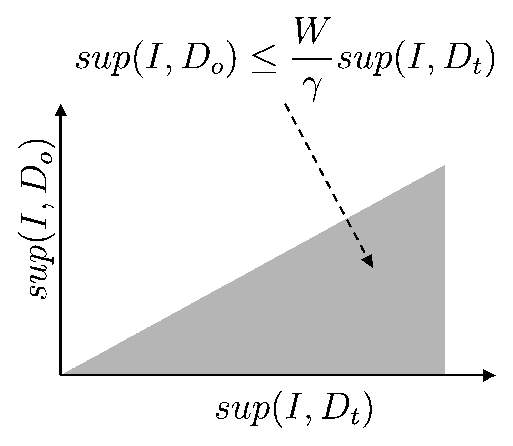
\includegraphics[scale=0.5]{./ep.eps}
\caption{顕在パターン\label{fig:ep}}
\end{center}
\end{minipage}

\begin{minipage}{0.3\hsize}
\begin{center}
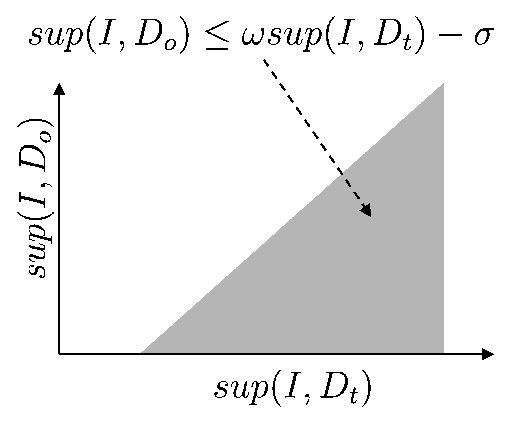
\includegraphics[scale=0.5]{./cp.eps}
\caption{コントラストパターン\label{fig:cp}}
\end{center}
\end{minipage}

\begin{minipage}{0.3\hsize}
\begin{center}
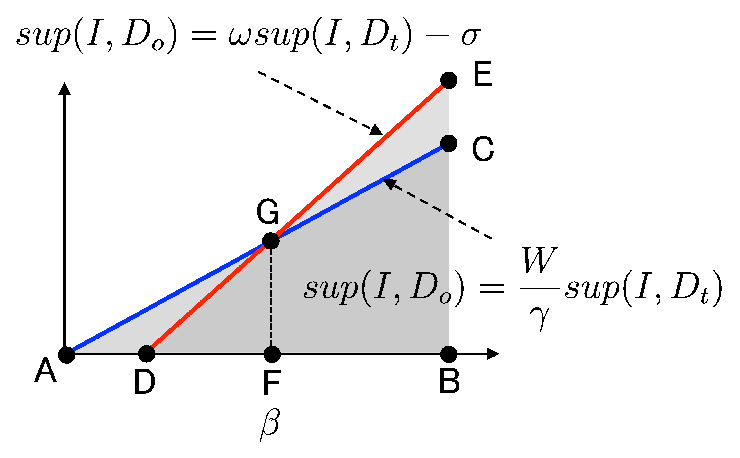
\includegraphics[scale=0.5]{./epcp.eps}
\caption{2つのパターンの関係\label{fig:epcp}}
\end{center}
\end{minipage}


\end{tabular} 
\end{center}
\end{figure} 

LCMでは,ユーザがパラメータ$\omega, \sigma$を与えることで
コントラストパターンを高速に列挙することができる.
コントラストパターンの列挙においては、$sup(I,D_t)$が大きくなればなるほど、
$sup(I,D_o)$との差が相対的に小さいパターンが列挙されることもあり、
そのようなパターンはクラス$c_t$に特徴的なパターンとは言えなくなる。
この欠点を回避するために、本コマンドでは顕在パターンの列挙を採用している。

ここで問題となるのは、コントラストパターンを列挙するLCMを使って、
いかに顕在パターンを列挙するかであり、以下に本コマンドで採用している方法を示す。

図\ref{fig:epcp}は、図\ref{fig:ep}と図\ref{fig:cp}を重ねた図である。
ここでは顕在パターンの領域ABCを全て列挙するのではなく、
$sup(I,D_t)\ge\beta$($\beta$は本コマンドS=で指定するパラメータ)を満たす領域GFCBに属する顕在パターンの列挙を考える。
LCMによって列挙されるパターンは、$\triangle{DEB}$に属するパターンであるが、
直線DEは、$\sigma$と$\omega$を定めることによって決まる。
まず$\sigma$は、直線ACと直線DEの交点Gの$x$座標が、ちょうど$\beta$になるように
設定する(式(\ref{sigma_beta}):$\omega$の決め方は後述)。
そうすることで、LCMが列挙した全パターンから、
$\triangle{DFG}$および$\triangle{EGC}$に属する
パターンを削除すれば、目的とする顕在パターンを列挙することが可能となる。

\begin{equation}
\sigma=\beta (\omega-\frac{W}{\gamma})  \label{sigma_beta}
\end{equation}



次に$\omega$であるが、これは直線DEの傾きを決めることに対応する。
一般的に$\triangle{EGC}$に属するパターンより、$\triangle{DGF}$に属するパターンの方が遥かに多いので、
$\omega$をできる限り大きくする方が効率的である。

しかしながら、$\omega$はトランザクションの重みであり、計算機上で件数をカウント
する変数の型の最大値に制約される。
その最大値を$maxInt$とすると、$\omega sup(I,D_t)\le maxInt$の制約を
満たしていなければならない。
$sup(I,D_t)$は$|D_p|$を超えることはないので、$\omega$を式(\ref{omega})のとおり
指定することで、$\triangle{DFG}$の列挙数を最小化できる。

\begin{equation}
\omega=\frac{maxInt}{|D_t|} \label{omega}
\end{equation}

